

\section{Introduction}
\label{sec:introduction}

\vspace{-1em} %This is a trick to avoid PDF links issues.

The quantitative understanding of the physical world is an essential goal of geoscience research. We use mathematical abstractions to represent the behavior of systems under static and dynamic conditions; and we define properties such as density and elastic moduli to characterize the capacity of materials to absorb or transmit forces in static and dynamic processes. In seismology and geophysics, our understanding of physical phenomena associated with earthquakes, their genesis, and effects, depends, in good measure, on our knowledge and accurate representation of the geometry and material properties of the Earth's structure, as well as on our capacity to represent the mechanical characteristics of the earthquake rupture process and the subsequent propagation of seismic waves through the earth. Computational geoscientists use stress conditions and dynamic rupture models to describe faulting processes, and seismic velocity and attenuation models, along with wave propagation principles, to calculate characteristics of earthquake ground motions. Initial stress models and seismic velocity models are therefore the basic input used in earthquake ground motion simulation.

We are interested in how seismic velocity models are built and made available to geoscientists, and how these models can help advance physics-based earthquake science. We utilize modeling approaches based on deterministic numerical techniques---such as the finite element, finite difference, or spectral element methods---to simulate the ground motion in ways that incorporate the physics of earthquake processes explicitly. That is, methods that explicitly solve the associated wave propagation problem. The use of physics-based earthquake simulation has increased considerably over the last two decades thanks to the growth in capacity and availability of high-performance computing (HPC) facilities and applications \citep[e.g.,][]{Aagaard_2008_BSSA2, Olsen_2009_GRL, Bielak_2010_GJI, Cui_2010_Proc}. These simulations have important applications in seismology and earthquake engineering for purposes such as the assessment of regional seismic hazard \citep[e.g.,][]{Graves_2011_PAG}.

Recent earthquake simulations have shown the importance of velocity models in the accuracy of simulation results \citep[e.g.,][]{Taborda_2014_BSSA}. Numerous seismic velocity models have been built for specific regional or local structures and used in particular simulations over the years \citep[e.g.,][]{Frankel_1992_BSSA, Brocher_2008_BSSA, Graves_2008_BSSA}. The concept of community velocity models (CVMs) has emerged from broad use of velocity models in earthquake simulations. CVMs are seismic velocity models that have been developed, maintained, improved, and used by a community of interested investigators. Some examples of CVMs for the regions of southern and northern California, Utah, and the central United States are those models developed by \citet{Kohler_2003_BSSA}, \citet{Suss_2003_JGR}, \citet{Brocher_2006_Proc}, \citet{Magistrale_2006_Tech}, \citet{Plesch_2011_SCEC}, and \citet{RamirezGuzman_2012_BSSA}. 

CVMs are typically distributed in the form of datasets or collections of files, or in the form of computer programs that can dynamically operate on these datasets and files to provide information about the geometry and material properties of the crust in a particular region. However, these datasets and computer programs have not been designed consistently from a computational perspective. For example, not all CVM's define the same material properties, or use the same geographical projection. In addition, recent advances in earthquake simulations, powered by the increasing capability of supercomputers, have increased significantly the computational demand placed on CVMs as input to these simulations.

This paper presents the Unified Community Velocity Model (UCVM), a software framework developed and maintained by the Southern California Earthquake Center (SCEC), designed to provide standardized and computationally efficient access to seismic velocity models. UCVM is a collection of software tools and application programming interfaces (APIs) that facilitate access to the material properties stored in CVMs. Although UCVM was conceived as a tool to aid physics-based earthquake ground-motion simulation and regional seismic hazard assessment, it can be, and has been used in other geoscience and engineering applications. Here, we describe the development of UCVM and its various software components and features, including its use in high-performance parallel computers, and present examples of recent applications of UCVM tools in geoscience and earthquake engineering research.



\section{Community Velocity Models}
\label{sec:cvms}

\textit{
\color{blue}
This section will present how CVMs work and the various CVMs available to the community today. It will basically explain that CVMs provide the triplets of Vs, Vp and density, and, as an example, we can expand on a description of CVM-S and CVM-H, including their variations CVM-SI and CVM-H+GTL.
}

\section{The UCVM Software Framework}\label{sec:ucvm}
The primary functionality provided by UCVM is the ability to query a wide array of community velocity models for material properties in a standard way. Once a velocity model has been successfully integrated with UCVM, the framework can be utilized to query for the primary and shear seismic wave velocities ($Vp$, $Vs$) as well as the soil/rock density ($\rho$) at any geographic point within that model. The original model's local coordinate system and map projection are concealed behind a generic interface that instead allows queries by geographic latitude and longitude along with a vertical z-coordinate. The z-axis may be defined as either depth below the free surface or elevation relative to mean sea level.

To support this flexible query mechanism consistently across all models, UCVM includes a high-resolution digital elevation model (DEM). The DEM is synthesized from the USGS National Elevation Dataset (TODO: cite USGS NED) and the ETOPO1 Global Relief Model (TODO: cite ETOPO1). It currently spans the State of California along with portions of surrounding States. However, it may be modified to cover any arbitrary region of the Earth's surface, provided adequate resolution elevation datasets exist. An additional advantage to providing the built-in DEM is that UCVM is able to return the surface elevation at any query point in addition to the traditional $Vp$, $Vs$, and $\rho$ parameters.
\begin{figure}
\centering
\epsfig{file=UCVM_Tiling_Concept.pdf,scale=0.35}
\caption{Tiling of velocity models (TODO: Redo/cleanup this figure).}\label{fig:tiling}
\end{figure}

The framework further extends the standardized interface by allowing multiple velocity models to be aggregated into a single composite model. Composition is accomplished by tiling two or more velocity models in three dimensions according to a user-specified priority ordering. Under this scheme, a query point is submitted sequentially to each velocity model within the ordered list that comprises the composite. The first model to return valid velocity data for the point is considered to have fulfilled the data request and subsequent models are not queried. Thus, overlap among the individual models is acceptable and their relative priority ordering arbitrates which one satisfies any given query. Generally, no smoothing is performed at the interfaces between models (an exception is interpolation between a geotechnical layer and a crustal model as discussed later in this paper). This tiling concept is illustrated in Figure \ref{fig:tiling}.

Community velocity models vary widely in their area of coverage, depth extent, and resolution. UCVM is flexible in its support for such variability. However, in order to better accommodate high frequency ground motion simulations, it categorizes models into two general groups: crustal models, and geotechnical layers (GTLs). Crustal models provide subsurface seismic wave velocities associated with basin, crust, and mantle structures. These models may potentially extend to many tens of kilometers below the Earth's surface yet do so at coarse resolutions (TODO: cite CVM-H, CVM-S). Geotechical layers, in contrast, provide velocities for only the near-surface (typically a few hundred meters) at very high resolution (TODO: cite Ely Vs30 GTL). Ground motion simulations, in particular, rely on high-resolution near-surface velocities and therefore a GTL serves to supplement the coarser data provided by crustal models.
\begin{figure}
\centering
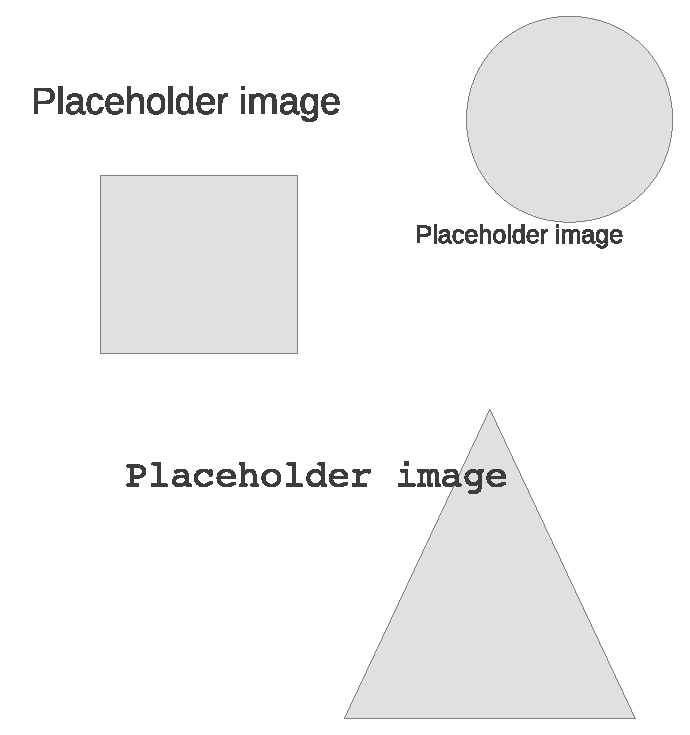
\epsfig{file=place_holder.pdf,scale=0.35}
\caption{Interpolation of GTL and crustal model.}\label{fig:interpolation}
\end{figure}

Whereas a set of velocity models consisting only of crustal models is aggregated by the tiling mechanism described above, a more sophisticated interpolation mechanism is employed if one or more GTLs are involved. The primary motivation for performing interpolation in this particular case is to eliminate near-surface discontinuities in the composite model which would adversely affect ground motion simulations. When a GTL is specified in the ordered list of models, the framework creates a default interpolation zone along the z-axis over which smoothing between this GTL and the underlying crustal models is performed. Query points that fall within the zone are assigned an interpolated velocity based on the GTL velocity at the top of the zone boundary and the crustal model velocity at the bottom. By default, linear interpolation is used for the smoothing but both the zone dimensions and interpolation function can be modified by the user. Figure \ref{fig:interpolation} illustrates how this interpolation is performed. 

A single geotechnical layer is currently supported, based on Ely's Vs30-derived algorithm (TODO: cite Ely Vs30-derived GTL). This algorithm procedurally estimates $Vp$, $Vs$, and $\rho$ from the Vs30 velocity at the point of interest. To that end, two separate Vs30 maps are provided for use with the Ely GTL, and each covers the same geographic region as the DEM (namely, California). One map is based on the the Wills and Walls dataset (TODO: cite Wills and Wald), and the other is based on the Yong dataset (TODO: cite Yong). Alternative Vs30 maps may be integrated as new datasets become available. As with the surface elevation from the DEM, the raw Vs30 value from the Vs30 map is returned by UCVM for each query point.

\subsection{Command-line Utilities}

\subsubsection{Querying}

TODO: command-line query

\subsubsection{Meshing}

TODO: single core and parallel meshing/etree extraction

\subsection{Application Programming Interface}

TODO: how to interface programmatically with UCVM

\subsubsection{Integrating New DEMs, Vs30 Maps, and Community Velocity Models}

TODO: describe how to support new DEMs, Vs30 maps, and models

\section{Computational Performance}
\label{sec:conclusions}

\textit{
\color{blue}
It would be desirable to do some experiments in terms of performance, especially for the parallel applications utilities in UCVM. With some examples of how long the same thing would take if doing it differently. We will need to discuss this.
}

\section{Recent Case Applications}
\label{sec:conclusions}

\textit{
\color{blue}
This section will be dedicated to show case applications. Some ideas for potential subsections follow.
}

\subsection{Visualization and Model Comparisons}

\subsection{Chino Hills Simulation Series}

\subsection{CyberShake}

\section{Summary and Conclusions}
\label{sec:conclusions}

\textit{
\color{blue}
A couple of paragraphs with a summary of what is shown in the paper and a few key conclusions about the impact that we expect UCVM has already have and will have on earthquake research.
}

